\section{Higgs Production Mechanisms} \label{sec:higgs:production}

At the LHC the dominant production mechanisms for the Higgs boson in order of
decreasing cross section are: gluon-fluon fusion (ggF), vector boson fusion
(VBF), vector boson associated production or ``Higgsstrahlung" (VH), and
associated production with $t\bar{t}$ ($t\bar{t}H$) and $b\bar{b}$
($b\bar{b}H$).  The cross sections for the signatures of these processes with
associated theoretical uncertainties for each are shown as a function of the
center-of-mass energy $\sqrt{s}$ in \Cref{fig:higgs_xsection}, and the
leading order (LO) Feynman diagrams can be seen in \Cref{fig:higgs_production}.

\begin{figure}[!htbp]
  \begin{center}
    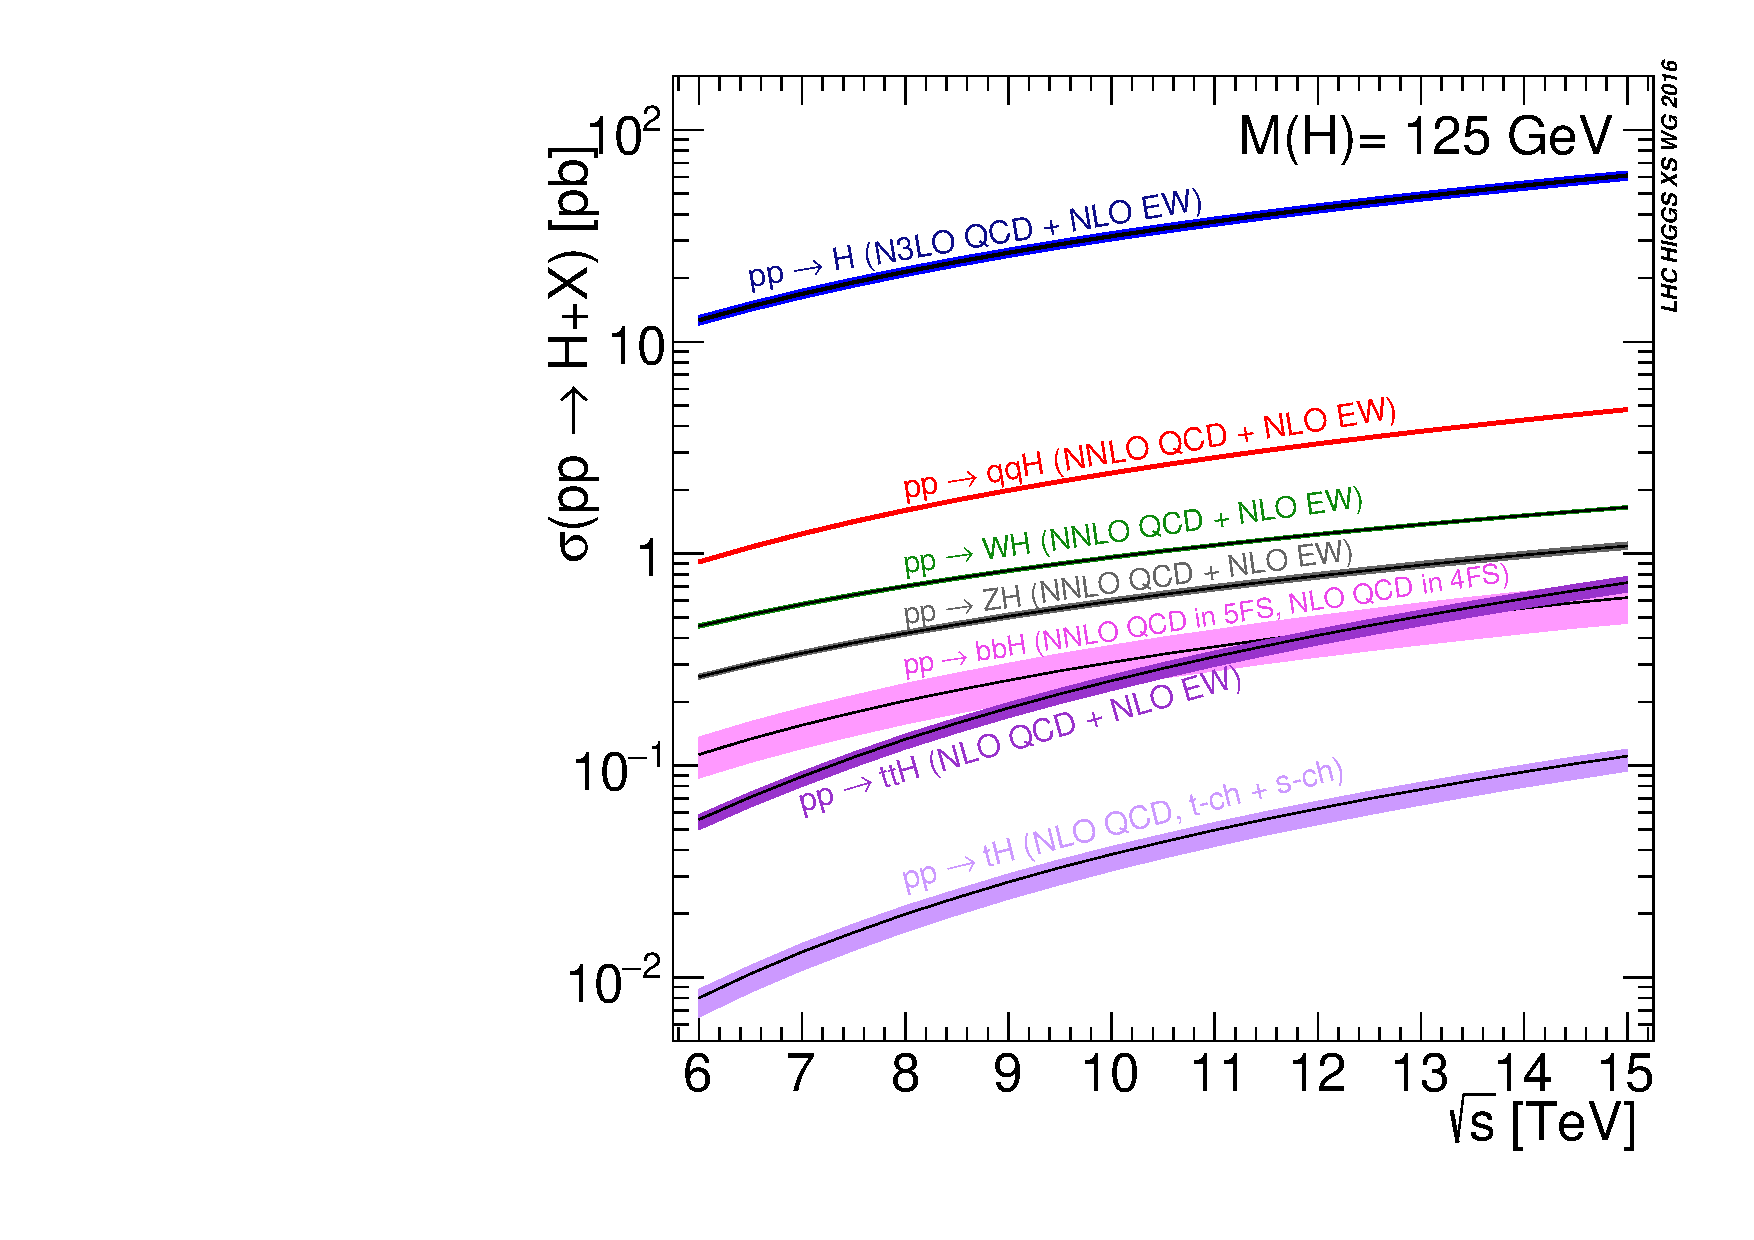
\includegraphics[width=0.5\linewidth]{figures/higgs/higgs_xsection.pdf}
    \caption{Cross sections for the production of the SM Higgs boson signatures
as a function of the center of mass energy ($\sqrt{s}$) at the LHC
\cite{PDG2018:Ch11}.  In order of decreasing cross section: the ggF process
signature is $H$, the VBF process signature is $qqH$, the VH process signature
is split into $WH$ and $ZH$, and the $b\bar{b}$ / $t\bar{t}$ signatures are
$t\bar{t}H$ / $b\bar{b}H$.}
    \label{fig:higgs_xsection}
  \end{center}
\end{figure}

The LO Feynman diagram contains the least number of vertices, and thus coupling
constants, making it the largest contribution to the cross-section calculation.
Adding an additional vertex, represents a higher order correction to the LO
calculation known as next-to-leading order (NLO) where each additional vertex
adds a ``next" (N2LO, N3LO, etc.). For reference, the current best
estimates of the production cross sections for the leading production
mechanisms are detailed in \Cref{table:higgs_production_xsection}.

\begin{figure}[!htbp]
\centering

\subcaptionbox{gluon-gluon fusion}{
\resizebox{0.48\textwidth}{!}{
\begin{tikzpicture}[thick]
 \begin{feynman}
  \vertex (origin);
  \vertex [right=1.5cm of origin] (H);
  \vertex [above left=1cm and 1.2cm of origin] (v1);
  \vertex [below left=1cm and 1.2cm of origin] (v2);
  \vertex [left=1.75cm of v1] (g1) {\(g\)};
  \vertex [left=1.75cm of v2] (g2) {\(g\)};
  \diagram* {
  (origin) -- [red, scalar, edge label={\(H\)}] (H),
  (origin) -- [fermion] (v1) -- [fermion] (v2) -- [fermion] (origin),
  (g1) -- [gluon] (v1),
  (g2) -- [gluon] (v2),
  };
 \end{feynman}
\end{tikzpicture}
}}
\subcaptionbox{vector boson fusion}{
\resizebox{0.48\textwidth}{!}{
\begin{tikzpicture}[thick]
 \begin{feynman}
  \vertex (origin);
  \vertex [right=1.5cm of origin] (H);
  \vertex [above left=1cm and 1.2cm of origin] (v1);
  \vertex [below left=1cm and 1.2cm of origin] (v2);
  \vertex [left=1.75cm of v1] (q1) {\(q\)};
  \vertex [left=1.75cm of v2] (q2) {\(q\)};
  \vertex [above right=0.25cm and 1.75cm of v1] (q3) {\(q'\)};
  \vertex [below right=0.25cm and 1.75cm of v2] (q4) {\(q'\)};
  \diagram* {
  (v1) -- [boson, edge label={\(V\)}] (origin),
  (origin) -- [boson, edge label={\(V\)}] (v2),
  (origin) -- [red, scalar, edge label={\(H\)}] (H),
  (q1) -- [fermion] (v1),
  (q2) -- [fermion] (v2),
  (v1) -- [fermion] (q3),
  (v2) -- [fermion] (q4),
  };
 \end{feynman}
\end{tikzpicture}
}} \\
\subcaptionbox{associated production}{
\resizebox{0.48\textwidth}{!}{
\begin{tikzpicture}[thick]
 \begin{feynman}
  \vertex (origin);
  \vertex [right=1.2cm of origin] (Vstar);
  \vertex [above right=0.50cm and 1.0cm of Vstar] (V1) {\(V\)};
  \vertex [red, below right=0.50cm and 1.0cm of Vstar] (H) {\(H\)};
  \vertex [above left=0.50cm and 1.0cm of origin] (g1) {\(\bar{q}\)};
  \vertex [below left=0.50cm and 1.0cm of origin] (g2) {\(q\)};
  \diagram* {
  (origin) -- [boson, edge label={\(V^{*}\)}] (Vstar) -- [boson] (V1),
  (Vstar) -- [red, scalar] (H),
  (origin) -- [fermion] (g1),
  (g2) -- [fermion] (origin),
  };
 \end{feynman}
\end{tikzpicture}
}}
\subcaptionbox{$t\bar{t}$ ($t\bar{t}H$) and $b\bar{b}$ ($b\bar{b}H$)}{
\resizebox{0.48\textwidth}{!}{
\begin{tikzpicture}[thick]
 \begin{feynman}
  \vertex (origin);
  \vertex [right=1.5cm of origin] (H);
  \vertex [above left=1cm and 0.2cm of origin] (v1);
  \vertex [below left=1cm and 0.2cm of origin] (v2);
  \vertex [left=1.75cm of v1] (g1) {\(g\)};
  \vertex [left=1.75cm of v2] (g2) {\(g\)};
  \vertex [above right=1.2cm and 1.4cm of origin] (t1) {\(t,b\)};
  \vertex [below right=1.2cm and 1.4cm of origin] (t2) {\(\bar{t},\bar{b}\)};
  \diagram* {
  (g1) -- [gluon] (v1),
  (g2) -- [gluon] (v2),
  (origin) -- [red, scalar, edge label={\(H\)}] (H),
  (origin) -- [fermion] (v1) -- [fermion] (t1),
  (t2) -- [fermion] (v2) -- [fermion] (origin),
  };
 \end{feynman}
\end{tikzpicture}
}}

\caption{Feynman diagrams representing the dominant Higgs production modes at
the LHC.}

\label{fig:higgs_production}
\end{figure}

\begin{table}[htpb]
 \centering
 \caption{ SM Higgs boson production cross sections in units of pb for
$m_{H}=125~\GeV$ in $pp$ collisions for the current LHC center-of-mass energy,
$\sqrt{s} = 13\TeV$.  The predictions for the ggF channel include the latest
N3LO results, which have reduced theoretical uncertainties by a factor around 2
compared to the N2LO results \cite{PDG2018:Ch11}.}
 \begin{tabular}{@{}rrrrrrrr@{}} \toprule
  $\sqrt{s}~(\TeV)$ & ggF                  & VBF                  & $WH$                 & $ZH$                 & $t\bar{t}H$            & Total~(pb) \\ \midrule
  \addlinespace[0.3em]
  $13$              & $48.6_{-5\%}^{+5\%}$ & $3.78_{-2\%}^{+2\%}$ & $1.37_{-2\%}^{+2\%}$ & $0.88_{-5\%}^{+5\%}$ & $0.50_{-13\%}^{+9\%}$ &  $55.1$    \\
  \addlinespace[0.3em]
  \bottomrule
 \end{tabular}\label{table:higgs_production_xsection}
\end{table}

The dominant Higgs production mechanism at hadron colliders is gluon-gluon
fusion.  This may seem strange as gluons are massless and thus do not couple
directly to the Higgs boson.  Instead the gluons indirectly couple to the Higgs
boson via a quark loop.  As discussed in \Cref{sec:theory:fermion_mass}, the
coupling of a fermion is proportional to $m_f$, so the dominant contribution to
this quark loop comes from the top quark. It is important to note that the ggF
cross section in \Cref{table:higgs_production_xsection} is inclusive in number
of final state jets and thus will include diagrams like the one shown in
\Cref{fig:h_plus_j}.  There has been considerable effort to calculate exclusive
$H$ + jet(s) production process at NLO and NNLO \cite{deFlorian:2016spz} for
use in analysis where there is an explicit requirement for an associated jet
such as the one presented in this dissertation in \Cref{part:HbbISR}.

\begin{figure}[!htbp]
\centering
\begin{tikzpicture}[thick]
 \begin{feynman}
  \vertex (origin);
  \vertex [right=1.5cm of origin] (H);
  \vertex [above left=1cm and 1.2cm of origin] (v1);
  \vertex [below left=1cm and 1.2cm of origin] (v2);
  \vertex [left=1.75cm of v1] (g1) {\(g\)};
  \vertex [left=1.75cm of v2] (g2) {\(g\)};
  \vertex at ($(g1)!0.5!(v1)$) (ISR_start);
  \vertex [above right=0.8cm and 1.5 cm of ISR_start] (ISR) {\(g\)};
  \diagram* {
  (origin) -- [red, scalar, edge label={\(H\)}] (H),
  (origin) -- [fermion] (v1) -- [fermion] (v2) -- [fermion] (origin),
  (g1) -- [gluon] (v1),
  (g2) -- [gluon] (v2),
  (ISR_start) -- [gluon] (ISR),
  };
 \end{feynman}
\end{tikzpicture}
\caption{Feynman diagram for ggF Higgs + jet production.}
\label{fig:h_plus_j}
\end{figure}

The second-largest cross section for Higgs production at the LHC comes from the VBF
mechanism.  In VBF the initial state quarks scatter via the exchange of a
$W^{\pm}$ or $Z$ boson which subsequently radiates the Higgs boson.  Unlike ggF
this production mechanism scatters the initial state quarks which allows them to
be observed as part of the interaction.  The presence of these extra quarks
makes these interactions easier to select during analysis.

The third-largest cross section for Higgs production is in association with a
vector boson. The cross section for this is even smaller than the above two, but
remains important due to the easily selected signature of the decaying vector
boson.  The largest background at the LHC is multijet events coming from
interactions that produce strong force objects.  Thus the leptons from the
boson's decay act as a discriminator against this multijet background greatly
reducing its effect on sensitivity. Note that the $W/Z$ can also decay
hadronically giving a final state that looks like $H$ + jet.

The lowest cross section of the four methods discussed is the
production of the Higgs boson in association with either $b\bar{b}$ or
$t\bar{t}$.  This channel is important because it allows direct measurement of
the $ttH$ coupling, unlike the ggF method where the quark in the loop is never
directly observed.
